\documentclass[12pt,oneside,a4paper,english]{article}
\usepackage[T1]{fontenc}
\usepackage[latin2]{inputenc}
\usepackage[margin=2.25cm,headheight=26pt,includeheadfoot]{geometry}
\usepackage[english]{babel}
\usepackage{listings}
\usepackage{color}
\usepackage{titlesec}
\usepackage{titling}
\usepackage[framed, numbered]{matlab-prettifier}
\usepackage{changepage}
\usepackage{amsmath}
\usepackage{hyperref}
\usepackage{enumitem}
\usepackage{graphicx}
\usepackage{fancyhdr}
\usepackage{lastpage}
\usepackage{caption}
\usepackage{tocloft}
\usepackage{setspace}
\usepackage{multirow}
\usepackage{titling}
\usepackage{float}
\usepackage{comment}
\usepackage{booktabs}
\usepackage{indentfirst}
\usepackage{lscape}
\usepackage{booktabs,caption}
\usepackage[flushleft]{threeparttable}
\usepackage[english]{nomencl}
\usepackage{xcolor}
\usepackage{lipsum}


% --- set footer and header ---
\pagestyle{fancy}
\fancyhf{}

\setlength{\parindent}{2em}
\title{Advanced Metrology} % to reference as \title, dont use \maketitle
\makeatletter\let\Title\@title\makeatother



\lstset{language=Matlab,
style=Matlab-editor,
basicstyle=\normalsize\mlttfamily,
numbers=left,
numberstyle={\scriptsize\color{black}},			% size of the numbers
numbersep=0.5cm											
}

\newlist{steps}{enumerate}{1}
\setlist[steps, 1]{leftmargin=1.5cm,label = Step \arabic*:}
\renewcommand{\headrulewidth}{1pt}
\renewcommand{\footrulewidth}{1pt}

%\lhead{\Title}
\rhead{\nouppercase{\rightmark}}
\lhead{\Title}
\rfoot{\includegraphics[height=1.25cm]{root/logo_long.png}} % right header logo
\setlength\headheight{16pt}
\setlength{\footskip}{50pt}
\lhead{\Title} %rightH title
\cfoot{\thepage}

% --- End of page settings ---



\begin{document}
\pagenumbering{roman} 

\begin{titlepage}
\begin{center}
\vspace{2cm}
\includegraphics[width=0.4\textwidth]{root/logo.png}~\\[1cm]
\vspace{2cm}

\vspace{2cm}

% Title
\hrule
\vspace{.5cm}
{ \huge \bfseries Advanced Metrology Report} % title of the report
\vspace{.5cm}

\hrule
\vspace{1.5cm}

\textsc{\textbf{Author}}\\
\vspace{.5cm}
\centering

% add your name here
Juan Manuel Boullosa Novo - 2481927\\

\vspace{4cm}

\centering Oldenburg, \today % Dags dato
\end{center}
\end{titlepage}

\newpage
\doublespacing
%\addcontentsline{toc}{section}{Table of Contents}
\renewcommand{\baselinestretch}{1}\normalsize
\tableofcontents
\renewcommand{\baselinestretch}{1}\normalsize
%\singlespacing
\thispagestyle{fancy} % force page style

\newpage
\pagenumbering{arabic} 
\fancyfoot[C]{Page \thepage\ of \pageref{EndOfText}}

\section{Introduction} \label{ch1}
In this document, I present the detailed analysis of data belonging to an emission and absorption spectral signal recorded using prism spectroscopy. This analysis was performed using Matlab. The analysis involves
several steps, beginning with a standard signal analysis to pre-process and clean the data. Then I performed a peak finding algorithm in order to identify the spectral lines. To obtain a better a better estimate of the continuum curve, I removed such peaks from it to create a calibration curve that allowed me to accurately fit a polynomial function and flatten the spectra.
Finally, I fitted Gaussian curves to the different peaks of the spectra in order to determine the element it belongs to, using the NIST database as a reference.

To carry out this analysis, I developed a Matlab tool with an accompanying Python script that fully automates the entire process and provide the necessary visualizations such as plots to aid with the result interpretation.  



\section{Basic data analysis} \label{ch1}
\subsection{Data outline}
In order to get a preliminary idea of the raw data, the 5 different values of the relative spectral intensity were plotted against the wavelength in nm,   as can be seen in \textbf{Figure \ref{fig:Figure 1}}.
\begin{figure}[H]
    \centering
    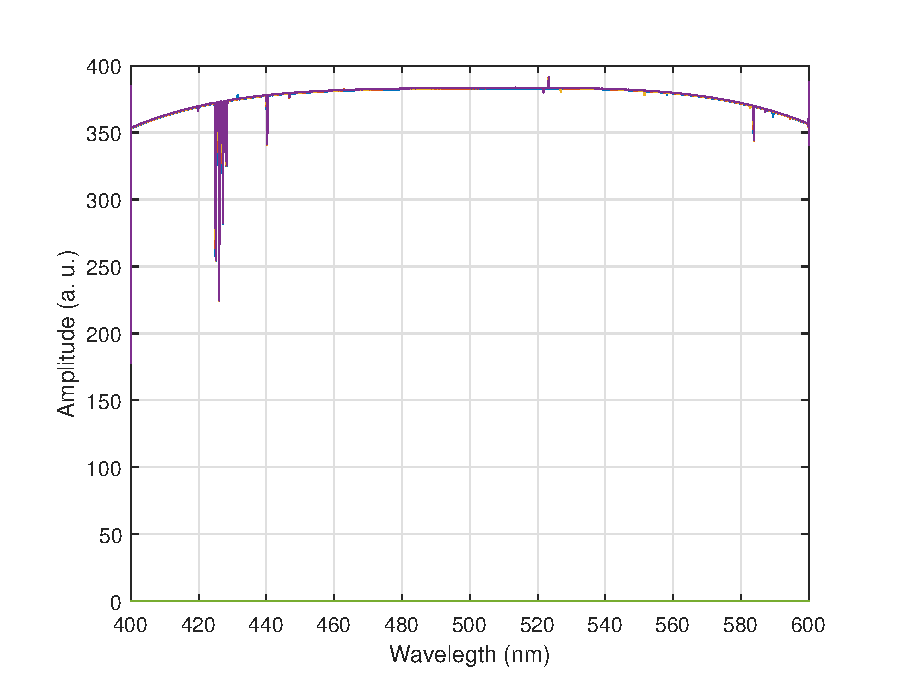
\includegraphics[width = 0.8\textwidth ]{figures/InitialPlot.eps}
    \caption{Initial plot. }
    \label{fig:Figure 1}
\end{figure}
Only 4 out of the 5 data-sets form the curve shown in the plot, as the 5th data-set is an array of broken data representing signal noise around the 0 intensity position. A zoomed out version of the data-set 5 can be seen in \textbf{Figure \ref{fig:Figure 2}}. This "broken" data was later used for noise estimations in the main spectrum. For the other four signals there is a presence of characteristic spectral peaks, both positive and negative, representing emission and absorption lines respectively. With the exception of a few spurious peaks, the majority appear consistently in each of the 5 data-sets, an example of some of these spurious peaks can be observed in \textbf{Figure\ref{fig:Figure 3}}. These also exhibit a measurable amount of random noise, as shown in \textbf{Figure \ref{fig:Figure 3}}, that is akin to the one observed in the 5th data-set. This noise can be due to spectrograph error, caused by variations in the light that goes through the prism and experimental noise\cite{Prisms}. Furthermore, there is a presence of strong intensity fluctuations around the first 10 and last 10 data-points in the spectrum. These are likely errors caused by the initiation and finalisation of the measurements, as seen in \textbf{Figure \ref{fig:Figure 4}}. After having determined this, a preliminary data cleanup is performed.


\begin{figure}[H]
    \centering
    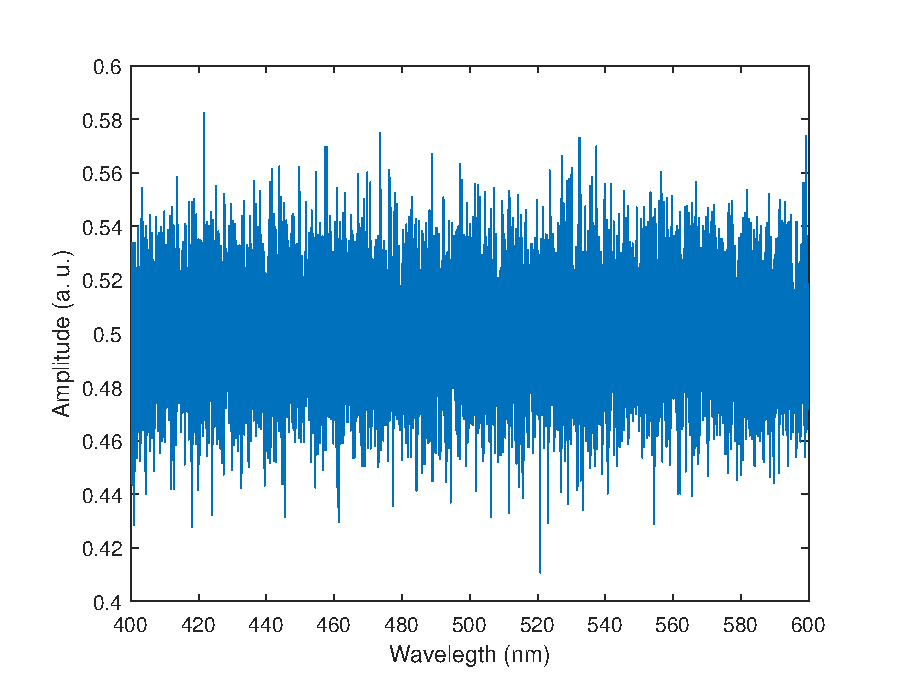
\includegraphics[width = 0.8\textwidth ]{figures/brokenData.eps}
    \caption{Broken data plot}
    \label{fig:Figure 2}
\end{figure}
\begin{figure}[H]
    \centering
    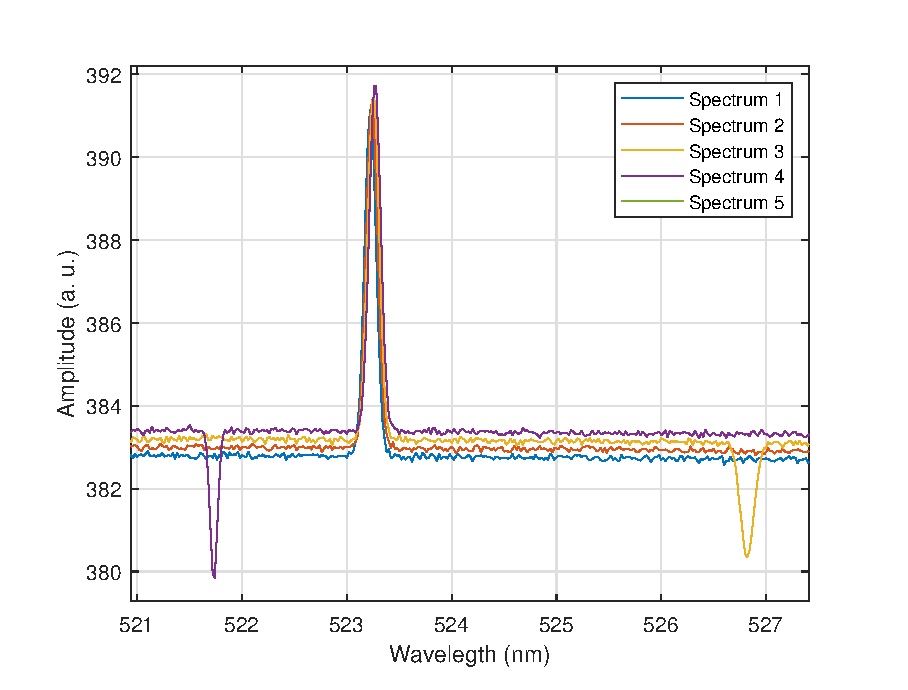
\includegraphics[width = 0.8\textwidth ]{figures/spurius_noise.eps}
    \caption{Spurious peaks and noise levels}
    \label{fig:Figure 3}
\end{figure}
\begin{figure}[H]
    \centering
    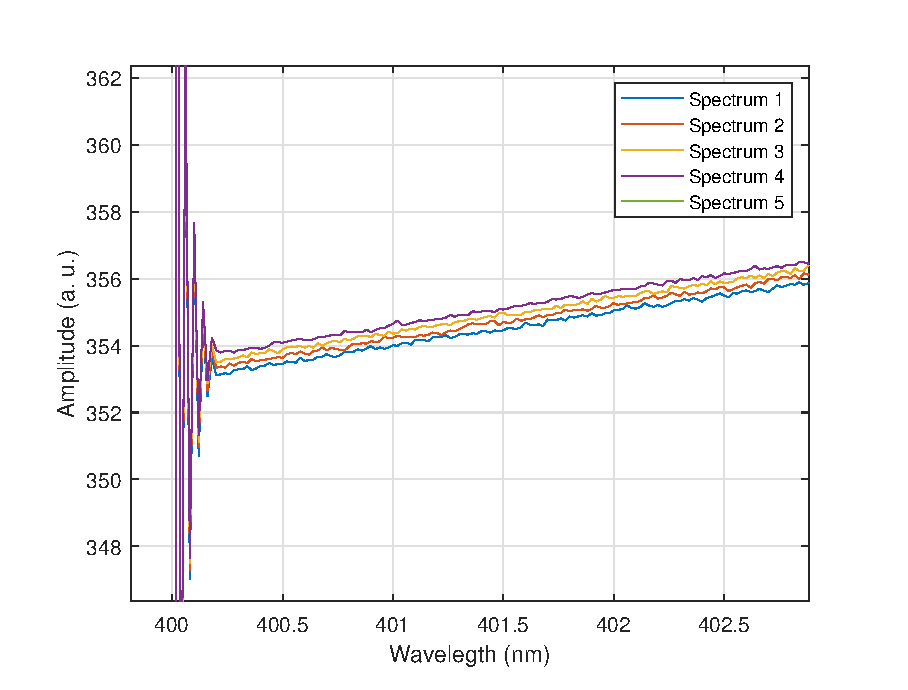
\includegraphics[width = 0.8\textwidth ]{figures/startError.eps}
    \caption{Start of measurement fluctuations}
    \label{fig:Figure 4}
\end{figure}
\subsection{Preliminary data processing}
First, the initialisation and finalisation fluctuation errors in the data are eliminated. For that, 12 points at the beginning of the data and at the end were removed, as a precaution measure to avoid interference with further data processing.


\subsection{Signal Characteristics}
The signal can be classified in different ways according to specific characteristics:
\begin{itemize}
    \item The signal is \textbf{deterministic}\cite{detSig}: The intensity of each wavelength in the emission spectrum depends on the specific conditions of the measurement and can be calculated precisely. This is despite random factors that cause uncertainty in the signal.
    \item The signal is \textbf{aperiodic}: The spectrum does not repeat itself or have a fixed time period
    \item The signal is \textbf{continuous}: The spectrum covers all wavelengths and is measured continuously without gaps or breaks
    \item The signal is \textbf{stationary}: The spectrum's properties are constant, showing equidistant samples at 0.02 nm.
    \item It is a \textbf{power signal}: The spectrum's intensity reflects the source's power output at each wavelength
    \item It is a \textbf{discrete-time signal}\cite{sigClas}:The values are at equally-spaced intervals along the x-axis.
\end{itemize}
\begin{table}[H]
    \centering
    \caption{Statistical properties of the signals (rounded up to 2nd decimal)}
    \begin{tabular}{|c|c|c|c|c|}
    \centering
    \textbf{} & \textbf{Mean} & \textbf{Var} &  \textbf{Skewness} & \textbf{Kurtosis}\\ \hline \hline
Spectrum 1   & 376.00    & 107.09    & -4.85 & 49.85 \\ \hline   
Spectrum 2   & 376.20    & 107.14    & -4.86 & 50.09 \\ \hline
Spectrum 3   & 376.39    & 107.06    & -4.86 & 50.09 \\ \hline
Spectrum 4   & 376.60    & 107.19    & -4.86 & 50.13 \\ \hline
Spectrum 5   & 0.5    & 4e-4    & 0.02 & 3.11
    \end{tabular}
    \label{tab:table1}
\end{table}
In \textbf{Table \ref{tab:table1}} can be observed basic statistical properties of the signal. As it can be observed, there is a continuous decrease of the Mean values in the signals for each data-set (excluding number 5). This could indicate a decrease in the luminous intensity perceived by the spectrograph in each subsequent measurement, perhaps even indicating that it has fallen out of range in measurement number 5. The variance, skewness and kurtosis do not show these differences and remain consistent across measurements. The variance indicates a dispersion in intensity across the whole spectrum, which includes the peaks of the spectral lines. This is the main source of the variance observed, as the residual noise is fairly small, as can be observed in the measurement number 5. The skewness is negative, indicating a general displacement of the higher intensities towards the lower wavelengths. This is also consistent with the higher peaks of the spectral lines that can be observed between 420 and 440 nm. The kurtosis values indicate substantial levels of peakness in the data, which are much more elevated than those of normal distributions, therefore proving that these sets of data-points are not normally distributed.

\subsection{Peak finding}
The spectral information from the data-sets 1 to 4 show a curvature, as observed in\textbf{ Figure \ref{fig:Figure 1}}. In order to accurately calculate the position of the spectral lines from these signals, this curvature has to be removed. In order to do that, a polynomial fit function that accurately describes the curvature has to be found, but Matlab 'polyfit' function showed inaccurate results due to the distorting effect of the spectral lines and other peaks in the data. Therefore, an algorithm for peak detection was used to identify and remove possible peaks from the continuum curve before fitting the polynomial. This algorithm returns the position and intensity of the peaks in all the spectra according to several parameters:

\begin{lstlisting}
numSpectra = 4; 
maxPeaksPerSpectrum = 10; % Pre-allocate space for performance
peaks = zeros(numSpectra, maxPeaksPerSpectrum);
peaksLoc = zeros(numSpectra, maxPeaksPerSpectrum);
negPeaks = zeros(numSpectra, maxPeaksPerSpectrum);
negPeaksLoc = zeros(numSpectra, maxPeaksPerSpectrum);

% Smooth the curve slightly for better 
% peak finding -currently 3-points moving average-
spectrum_smooth = smoothdata(spectrogram, 2, 'movmean', 3);

for i = 1:numSpectra
    % Find positive peaks in the spectrum
    [peaksFound, loc_posPeaks] = findpeaks(spectrum_smooth(i,:), 'MinPeakProminence', 0.5,'MinPeakHeight', 377.95,'Threshold', 0.02);
    numPeaksFound = numel(peaksFound);
    peaks(i, 1:numPeaksFound) = peaksFound;
    peaksLoc(i, 1:numPeaksFound) = loc_posPeaks;
        
    % Find negative peaks in the spectrum
    [negPeaksFound, loc_negPeaks] = findpeaks(-spectrum_smooth(i,:), 'MinPeakProminence', 0.2, 'Threshold', 0.005);
    numNegPeaksFound = numel(negPeaksFound);
    negPeaks(i, 1:numNegPeaksFound) = -negPeaksFound;
    negPeaksLoc(i, 1:numNegPeaksFound) = loc_negPeaks;
end
\end{lstlisting}
The results of the plotting can be observed in the \textbf{Figure \ref{fig:Figure 5}}.

\begin{figure}[H]
    \centering
    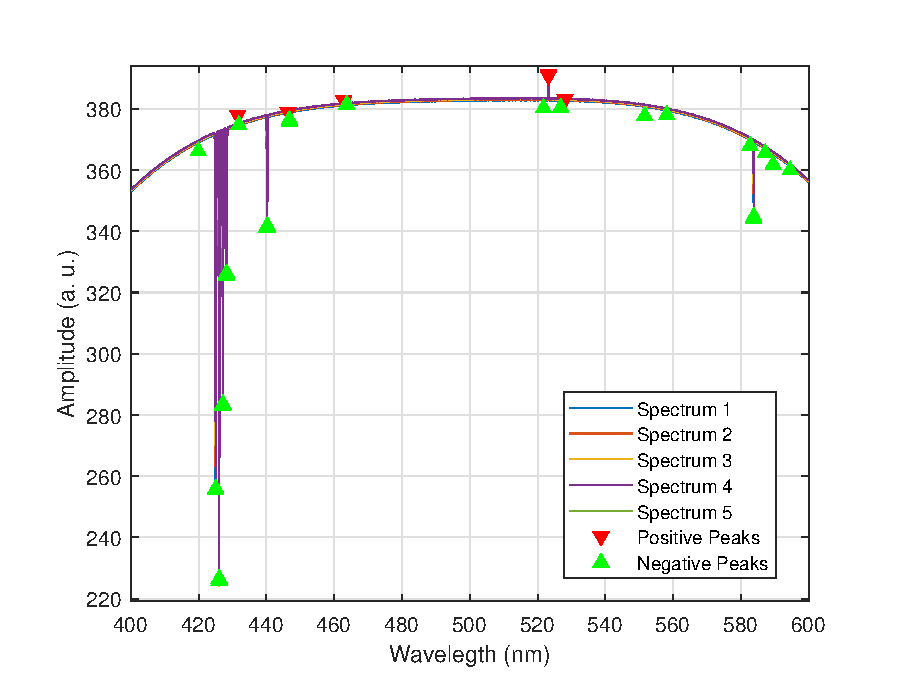
\includegraphics[width = 1\textwidth ]{figures/peakDetection1.eps}
    \caption{Location of detected peaks }
    \label{fig:Figure 5}
\end{figure}

\subsection{Calibration curve}
Based on the position of the peaks calculated in previous chapter, The continuum curve is split up into segments by removing a region of around 25 points before and after the peak maximum. The resulting data without the peaks is the calibration curve used to find the polynomial fit function for the spectra.
This curve is only used for finding the polynomial fit, and will not be used again elsewhere in the analysis.
The following Matlab algorithm was used:
\begin{lstlisting}
region_size = round(0.5 / wavelength_resolution);

for i = 1:numSpectra
    % Get the positive and negative peak locations for the current spectrum
    peak_locs = peaksLoc(i,:);
    peak_locs = peak_locs(peak_locs~=0); % Remove zero entries
    neg_peak_locs = negPeaksLoc(i,:);
    neg_peak_locs = neg_peak_locs(neg_peak_locs~=0); % Remove zero entries

    % Set values around the positive peaks to NaN in calibration_curve
    for j = 1:length(peak_locs)
        peak_loc = peak_locs(j);
        lower_bound = max(1, peak_loc - region_size);
        upper_bound = min(size(calibration_curve, 2), peak_loc + region_size);
        calibration_curve(i, lower_bound:upper_bound) = NaN;
    end
    
    % Set values around the negative peaks to NaN in calibration_curve
    for j = 1:length(neg_peak_locs)
        neg_peak_loc = neg_peak_locs(j);
        lower_bound = max(1, neg_peak_loc - region_size);
        upper_bound = min(size(calibration_curve, 2), neg_peak_loc + region_size);
        calibration_curve(i, lower_bound:upper_bound) = NaN;
    end
end
\end{lstlisting}
The visualisation of the calibration curve is in the following figure:(\textbf{Figure \ref{fig:Figure 6}})
\begin{figure}[H]
    \centering
    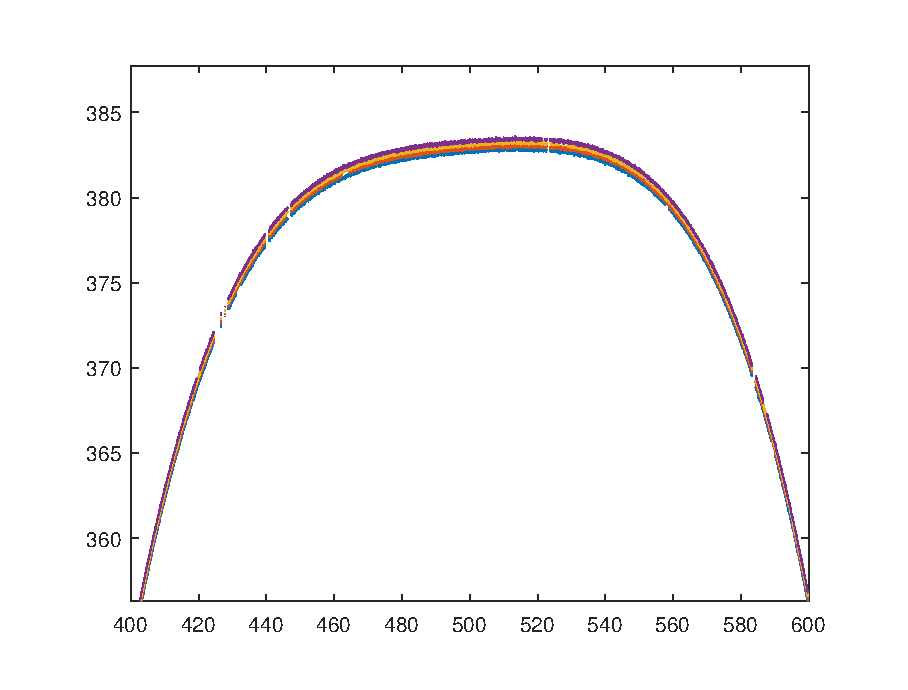
\includegraphics[width = 1\textwidth ]{figures/calibrationCurve.eps}
    \caption{Calibration Curve }
    \label{fig:Figure 6}
\end{figure}

Then, the empty gaps on the continuum are filled up by interpolating the empty values using interp1 linear interpolation as follows:
\begin{lstlisting}
current_row(nan_indices) = interp1(non_nan_indices, current_row(non_nan_indices), nan_indices, 'linear');
\end{lstlisting}
The result is a fully continuous curve (\textbf{Figure \ref{fig:Figure 7}}).
\begin{figure}[H]
    \centering
    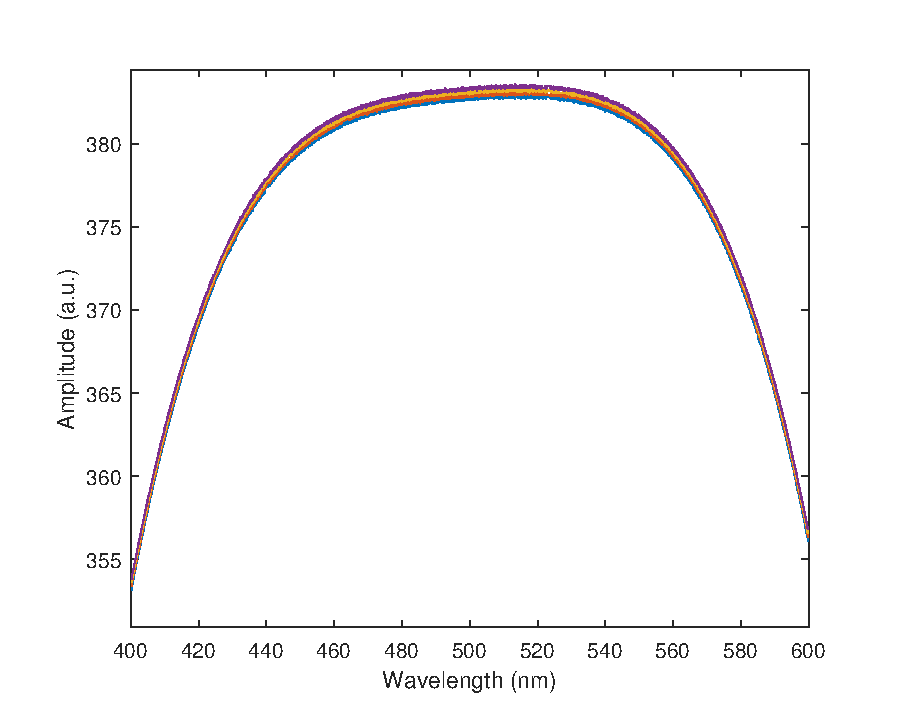
\includegraphics[width = 1\textwidth ]{figures/interpol_calibrationCurve.eps}
    \caption{Calibration Curve Interpolated }
    \label{fig:Figure 7}
\end{figure}

\subsection{Polynomial fit}
A polynomial fit of 4th degree is performed on the interpolated calibration curve. This allow us to obtain the parameters of the curve to correct the curvature of the signal. The following function 'polyfit'\cite{polyfit} was called in Matlab, and the results can be seen in \textbf{Figure \ref{fig:Figure 8}} as well as a zoomed-in version in \textbf{Figure \ref{fig:Figure 9}}.
\begin{lstlisting}
degree = 4;
p = polyfit(x(~isnan(y)), y(~isnan(y)), degree);
y_fit = polyval(p, x);
\end{lstlisting}
\begin{figure}[H]
    \centering
    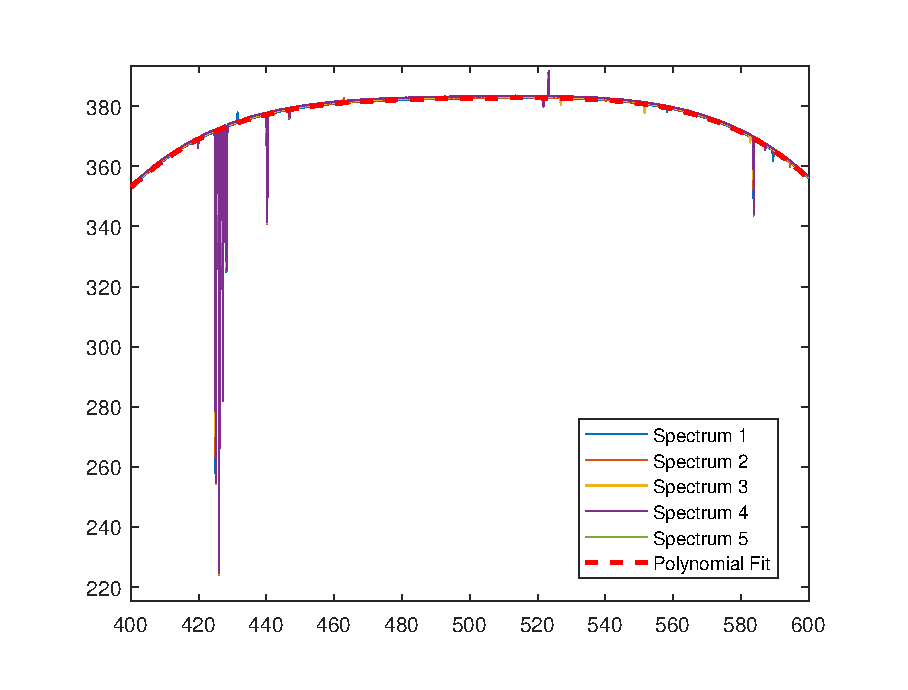
\includegraphics[width = 0.8\textwidth ]{figures/polyfit.eps}
    \caption{Polynomial fit of 4th degree on the calibration curve}
    \label{fig:Figure 8}
\end{figure}
\begin{figure}[H]
    \centering
    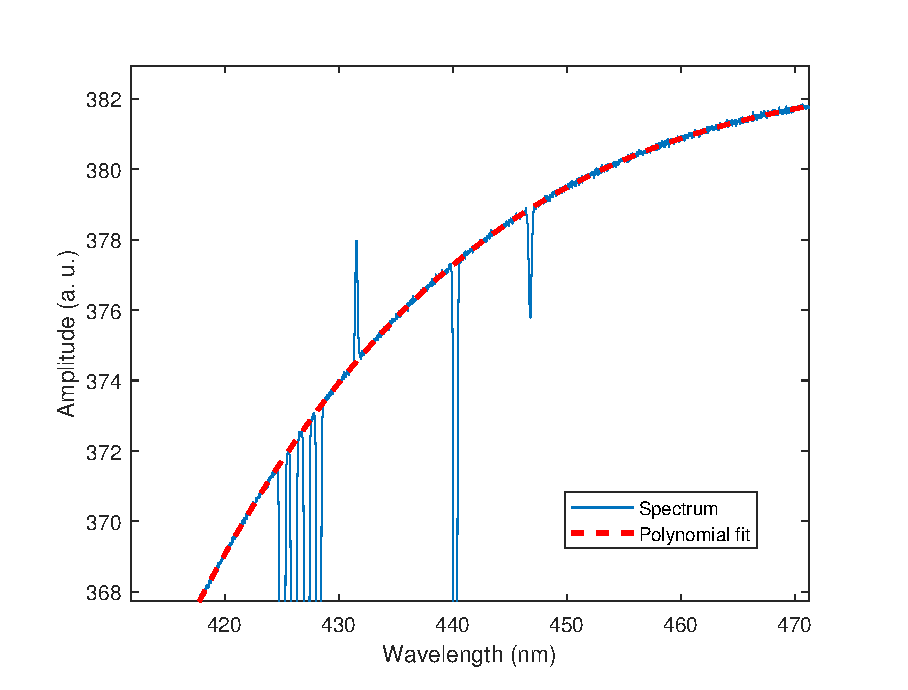
\includegraphics[width = 0.8\textwidth ]{figures/polyfit_zoom.eps}
    \caption{Polynomial fit zoom }
    \label{fig:Figure 9}
\end{figure}

\subsection{Curvature correction}
In order to correct the curvature of the continuum, I divided the entirety of the spectral data by the polynomial fit function. Then I detrended the signal by dividing it against its mean. This created a new corrected data for the 4 spectra, centered around 0, and can be observed in \textbf{Figure \ref{fig:Figure 10}}.

\begin{lstlisting}
corrected_signal = spectrogram ./ y_fit;
corrected_signal_detrended = bsxfun(@minus, corrected_signal, mean(corrected_signal, 2));
\end{lstlisting}

\begin{figure}[H]
    \centering
    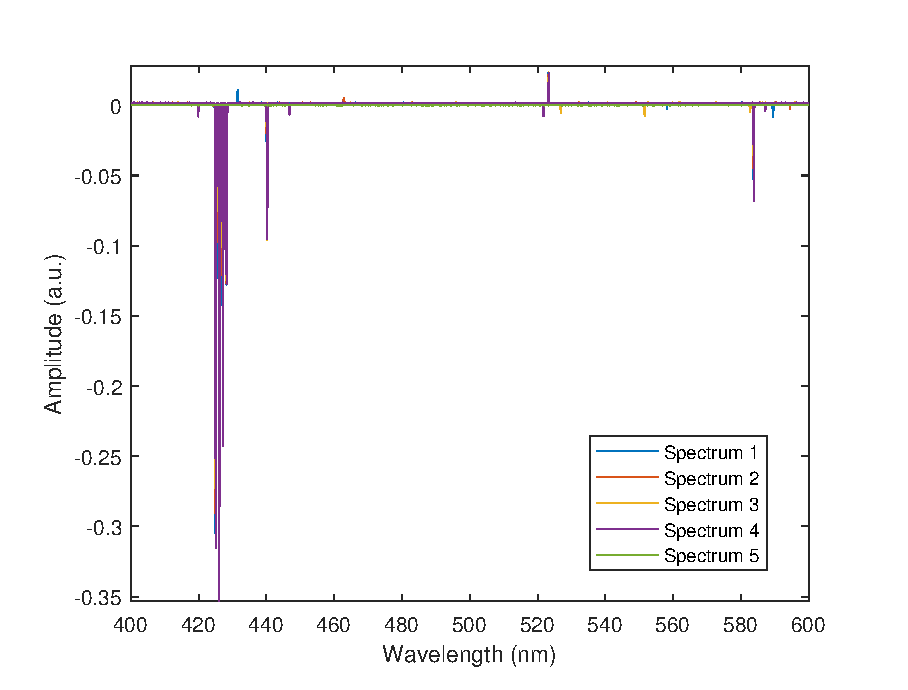
\includegraphics[width = 1\textwidth ]{figures/correctedSignal_detrended.eps}
    \caption{Corrected signal detrended}
    \label{fig:Figure 10}
\end{figure}

\subsection{Noise removal}
As mentioned in the Data outline, the data set number 5 contains seemingly broken data, but this could still be useful as it carries information about the background noise of the signals. This poses as an opportunity to further clean-up the spectral data of any random noise with the purpose to more accurately identify the spectral lines for element identification later on. Therefore I developed an algorithm to perform this cleaning.

\begin{itemize}
\item Subtracting the mean of data-set 5 from the rest of spectra
    \begin{lstlisting}
    cleaned_spectra = spectra - mean(spectra(5,:));
    \end{lstlisting}
    \item Calculate the noise threshold by obtaining absolute values of the data-set 5 and summing up the means
    \begin{lstlisting}
noise_threshold = max(abs(spectra(5,:)))+mean(cleaned_spectra(1:4,:),1)
\end{lstlisting}
    \item Set any values below the noise threshold to zero
    \begin{lstlisting}
for i=1:size(cleaned_spectra,1)-1
        for j=1:size(cleaned_spectra,2)
            if abs(cleaned_spectra(i,j)) < noise_threshold(i)
                cleaned_spectra(i,j) = 0;
            end
        end
    end
\end{lstlisting}
\end{itemize}

I also removed the spurious peaks such as the one shown in \textbf{Figure \ref{fig:Figure 3}}, by finding the peaks only present in one data-set, and setting them to zero.

\begin{lstlisting}
single_nonzero_cols = find(sum(cleaned_spectra(1:4,:)~=0,1)==1);
cleaned_spectra(1:4,single_nonzero_cols) = 0;
\end{lstlisting}

This results in a very clean signal in which the peaks of the spectral lines can be easily identified, as seeing in the detail against the previous noisy data in \textbf{Figure \ref{fig:Figure 11}}.

\begin{figure}[H]
    \centering
    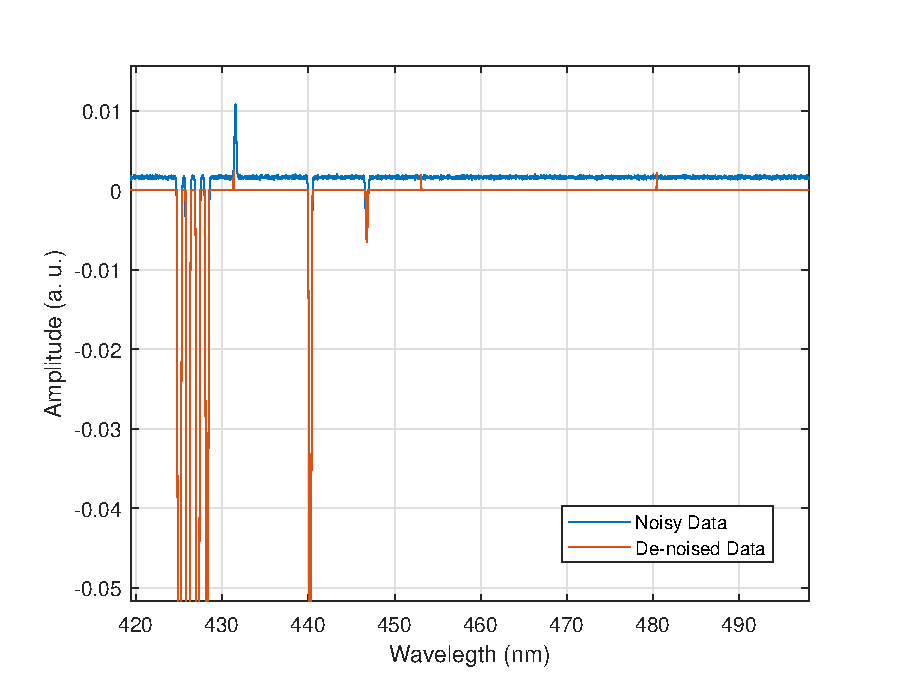
\includegraphics[width = 1\textwidth ]{figures/cleanedUpSpectra.eps}
    \caption{Cleaned-up data detail}
    \label{fig:Figure 11}
\end{figure}
\section{Advanced data analysis} \label{ch1}
\subsection{Gaussian fit for spectral lines}
In order to accurately determine the wavelength of the different spectral lines, every peak was identified from the clean data and then fitted by a Gaussian\cite{Gaussian} function. The formula used is described here:

\begin{equation} \label{eqn}
	f(x)=A\cdot \mathrm{e}_{}^{\frac{-1}{2}\cdot\left( \frac{x-b}{c} \right)^{2}}
\end{equation}

\begin{itemize}
    \item A describes the amplitude of the curve (maximum intensity)
    \item b describes the middle position of the curve (corresponds to peak wavelength)
    \item c describes the standard deviation of the curve
\end{itemize}

After every peak is identified in the clean data, the Gaussian fit function was used in Matlab as per below for every one of the 8 spectral lines identified in each of the 4 spectra. The result for the first spectral line of the first data-set is plotted in \textbf{Figure \ref{fig:Figure 12}}. The rest of the Gaussian fit plots can be found in the Appendix[\ref{fig:Figure 13}]. Also general information about the average values of the peaks obtained are in the \textbf{Table \ref{tab:table2}} and\textbf{ Table \ref{tab:table3}} below. There is a general error of 0.02 nm in the wavelength values due to the sample resolution of the wavelengths, or distance between points in the x-axis being 0.02 nm.

\begin{lstlisting}
    ft = fittype( 'gauss1' );
    opts = fitoptions( 'Method', 'NonlinearLeastSquares' );
    [fitresult, gof] = fit( xData, yData, ft, opts );
\end{lstlisting}

\begin{figure}[H]
    \centering
    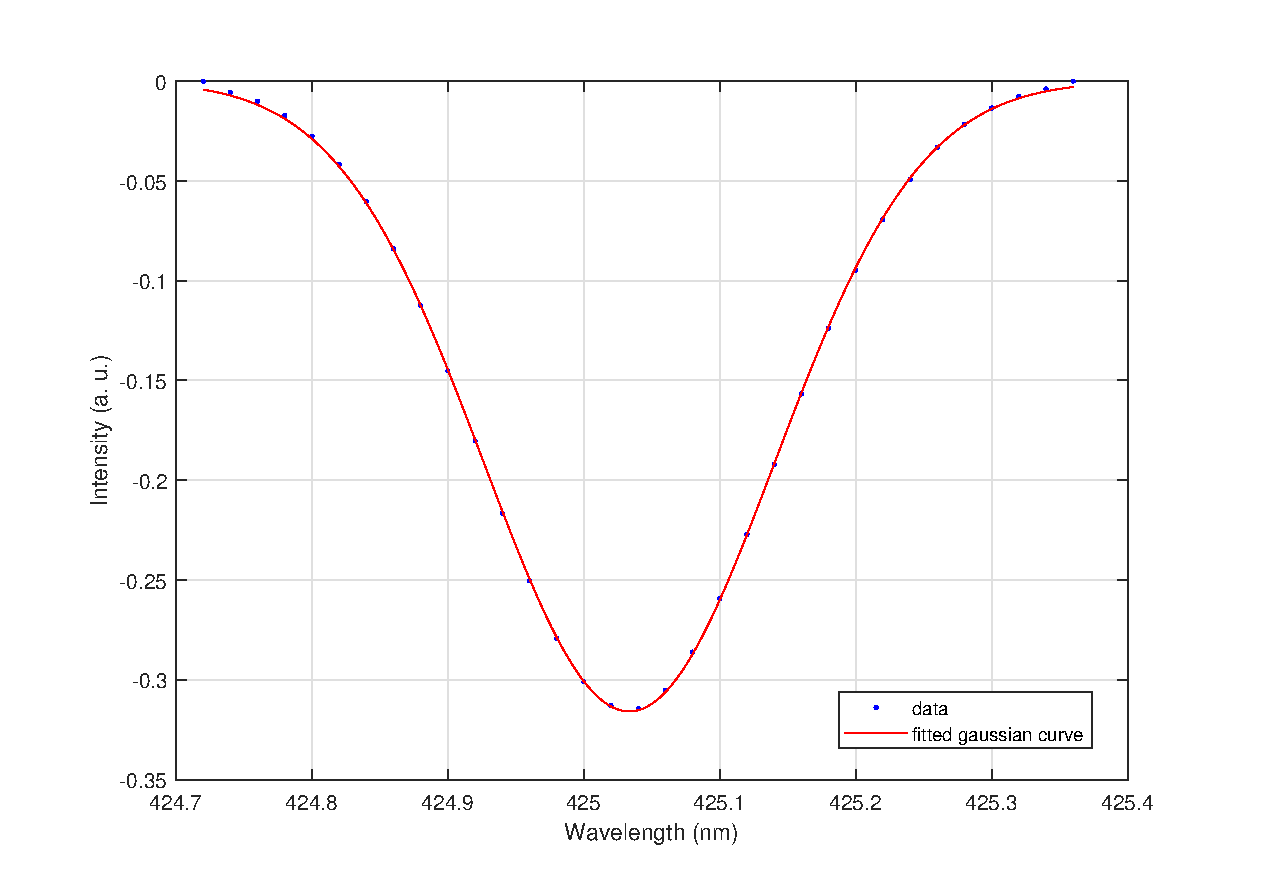
\includegraphics[width = 1\textwidth ]{figures/gauss_1.eps}
    \caption{Gaussian fit for spectral line 1 of spectrum 1 }
    \label{fig:Figure 12}
\end{figure}


\begin{table}[H]
    \centering
    \caption{Average maximum intensity of the peaks}
    \begin{tabular}{|c|c|c|c|c|c|c|c|c|}
    \centering
    \textbf{}   & \textbf{Line 1} & \textbf{Line 2} &  \textbf{Line 3} & \textbf{Line 4} & \textbf{Line 5} & \textbf{Line 6} & \textbf{Line 7} & \textbf{Line 8}\\ \hline \hline
    Spectrum 1   & -0.3158    & -0.3968    & -0.2430 & -0.1282  & -0.0961 & -0.0069 & 0.0234 & -0.0686 \\ \hline   
    Spectrum 2   & -0.3158    & -0.3977    & -0.2430 & -0.1282  & -0.0961 & -0.0069 & 0.0232 & -0.0685\\ \hline
    Spectrum 3   & -0.3157    & -0.3976    & -0.2429 & -0.1282  & -0.0960 & -0.0068 & 0.0233 & -0.0685\\ \hline
    Spectrum 4   & -0.3158    & -0.3981    & -0.2430 & -0.1281  & -0.0961 & -0.0070 & 0.0233 & -0.0684\\ \hline
   \textbf{Average}   & \textbf{-0.3158}    & \textbf{-0.3976}    & \textbf{-0.2430} & \textbf{-0.1282}  & \textbf{-0.0961} &\textbf{ -0.0069} & \textbf{0.0233} & \textbf{-0.0685}
    \end{tabular}
    \label{tab:table2}
\end{table}

\begin{table}[H]
    \centering
    \caption{Average wavelength of the Gaussian peak maximum (nm), with error tolerance of $\pm 0.02 nm$}
    \begin{tabular}{|c|c|c|c|c|c|c|c|c|}
    \centering
    \textbf{}   & \textbf{Line 1} & \textbf{Line 2} &  \textbf{Line 3} & \textbf{Line 4} & \textbf{Line 5} & \textbf{Line 6} & \textbf{Line 7} & \textbf{Line 8}\\ \hline \hline
    Spectrum 1   & 425.02    & 426.04    & 427.18 & 428.24  & 440.20 & 446.76 & 523.22 & 583.72 \\ \hline   
    Spectrum 2   & 425.04    & 426.06    & 427.18 & 428.24  & 440.22 & 446.78 & 523.24 & 583.74\\ \hline
    Spectrum 3   & 425.06    & 426.08    & 427.20 & 428.26  & 440.24 & 446.80 & 523.24 & 583.76\\ \hline
    Spectrum 4   & 425.08    & 426.08    & 427.22 & 428.28  & 440.24 & 446.80 & 523.26 & 583.78\\ \hline
    \textbf{Average}     & \textbf{425.06}    & \textbf{426.06}    & \textbf{427.20} & \textbf{428.26}  & \textbf{440.22} & \textbf{446.80} & \textbf{523.24 }& \textbf{583.76}
    \end{tabular}
    \label{tab:table3}
\end{table}

\subsection{Element determination for spectral lines}
After determining the average peak wavelengths of each spectral line and their intensity, 4 of those lines towards the lower end of the spectrum were selected and compared against an online database from the website of the National Institute of Standards and Technology (\textbf{NIST})\cite{NIST} (https://www.nist.gov/pml/atomic-spectra-database). For this purpose, a companion script written in Python was made to connect to the API of NIST, query and download the required data.
The script parses command-line data and generates a URL that then uses to extract data regarding the specific wavelengths in the range, element names and relative intensities of the spectral lines in question and saves the data to csv files to be read by matlab. Information on how to use it can be found in comments inside the script.
\begin{lstlisting}
API_NIST_v3.py

# Example usage:
#
# python.exe .\API_NIST_v3.py 426.5 data --element Fe --n 10 --low_w 425 --high_w 584 --ion_num 1 2 --min_intensity 10
\end{lstlisting}
After the query is complete, another matlab function loads the data (if it wasn't saved already), cleans it up, eliminating repeated rows, and identifies the most likely element according to the given wavelengths and intensities. This is done by looping over all spectral lines in the database and calculating the error by calculating the square difference between those values and the averages of the spectral lines' wavelengths calculated earlier.

\begin{lstlisting}
% Loop over each element in NIST_data_unique
    for i = 1:size(NIST_data_unique, 1)
        % Calculate the error between the current element and x_peaks/x_peaks_max
        error1 = sum((wavelengths(i) - x_peaks).^2);
        % error2 = sum((intensities(i) - x_peaks_max).^2);
        error = error1 + error2;
        
        % Update the closest match if the error is smaller than the current minimum
        if error < min_error
            min_error = error;
            matched_index = i;
        end
    end
    matched_element = NIST_data_unique(matched_index, 1);
\end{lstlisting}

As a result it returns the element with the lowest error value.
In this particular case, the identified element was \textbf{Chromium (Cr)}, with a match error score of: 5.7832, although other elements came close, such as Iron (Fe) with a score of 5.7886, and Actinium (Ac), with a score of 5.7877, despite being unlikely due to it being a rare metal.
 
\section{Conclusion} \label{ch1}
In conclusion, the analysis of the spectral lines data with Matlab and the cleaning up of the data of the 4 spectra has allowed for a more accurate determination of the peak locations of the spectral lines. By identifying the signal characteristics and finding the peaks to take away from the continuum curve, a polynomial function was able to be fit to flatten the curve, resulting in more precise peak measurements. Additionally, the fitting of Gaussian curves to the spectral lines provided more detailed information about their characteristics, which were then compared to the NIST database values. Through this process, it was determined that the spectral lines belonged to the element chromium. Overall, This study demonstrates the significance of meticulous data analysis in accurately characterizing spectral lines and identifying the elements that produce them. 

\label{EndOfText}

\newpage
\pagenumbering{Roman} 
\addcontentsline{toc}{section}{List of Figures}
\fancyfoot[C]{Page \thepage\ of \pageref{endOfDoc}}
\listoffigures
\thispagestyle{fancy}

\newpage
\addcontentsline{toc}{section}{List of Tables}
\listoftables
\thispagestyle{fancy}

\newpage
\addcontentsline{toc}{section}{References}
\bibliography{document.bib} 
\bibliographystyle{ieeetr}


\newpage
\section{Appendix} \label{ch6}
\begin{figure}[H]
    \centering
    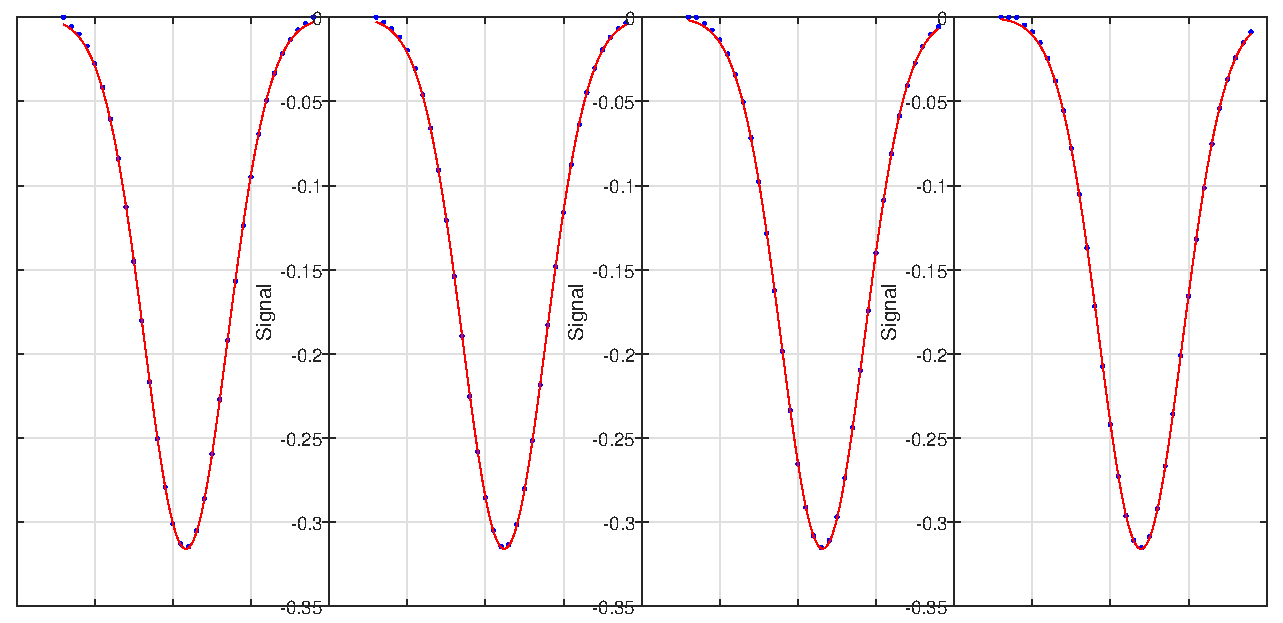
\includegraphics[width = 1\textwidth ]{figures/gaus_sl_1.eps}
    \caption{Gauss Spectral line 1.(absorption) }
    \label{fig:Figure 13}
\end{figure}
\begin{figure}[H]
    \centering
    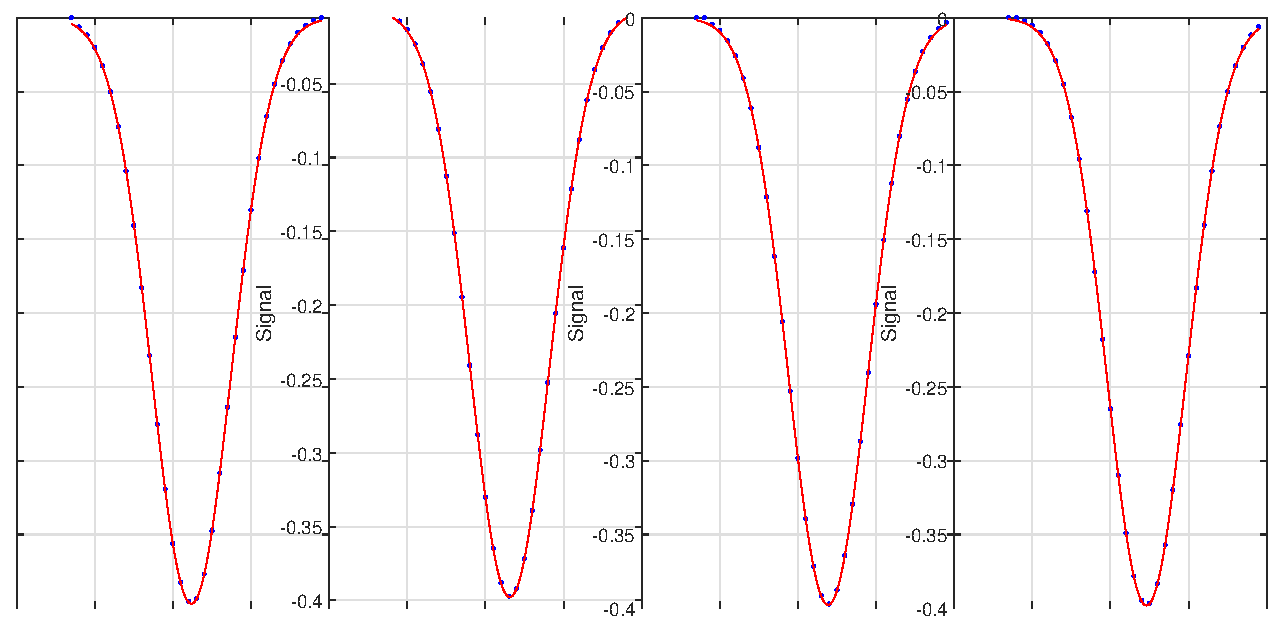
\includegraphics[width = 1\textwidth ]{figures/gaus_sl_2.eps}
    \caption{Gauss Spectral line 2.(absorption) }
    \label{fig:Figure 14}
\end{figure}
\begin{figure}[H]
    \centering
    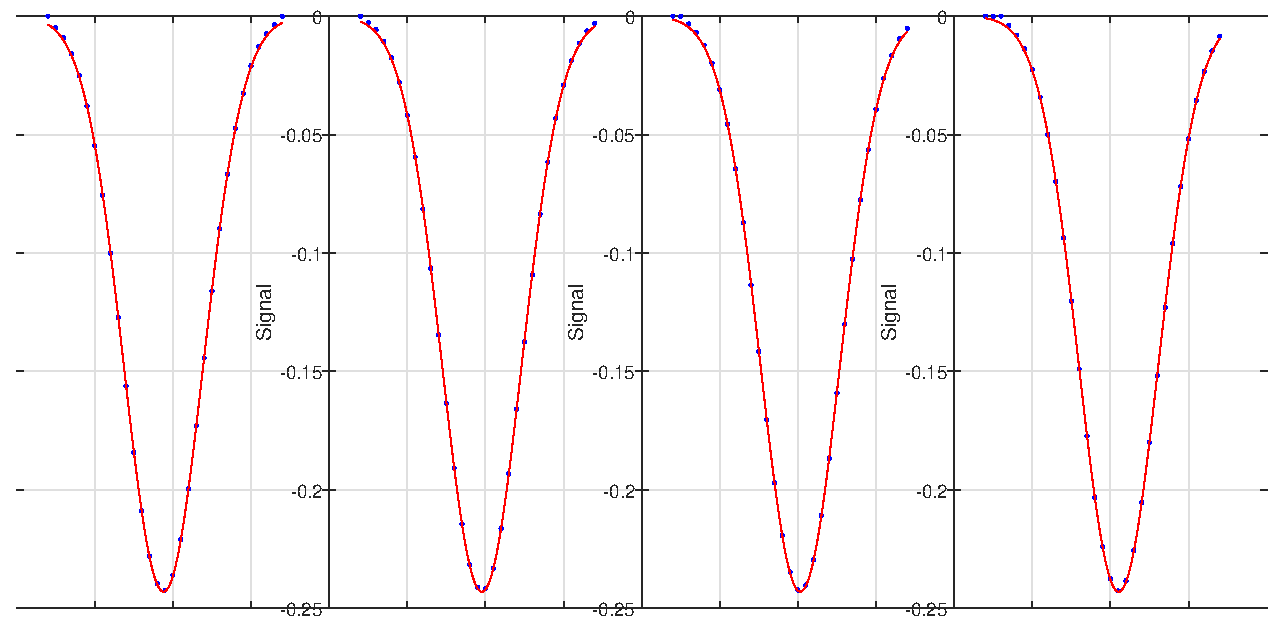
\includegraphics[width = 1\textwidth ]{figures/gaus_sl_3.eps}
    \caption{Gauss Spectral line 3.(absorption) }
    \label{fig:Figure 15}
\end{figure}
\begin{figure}[H]
    \centering
    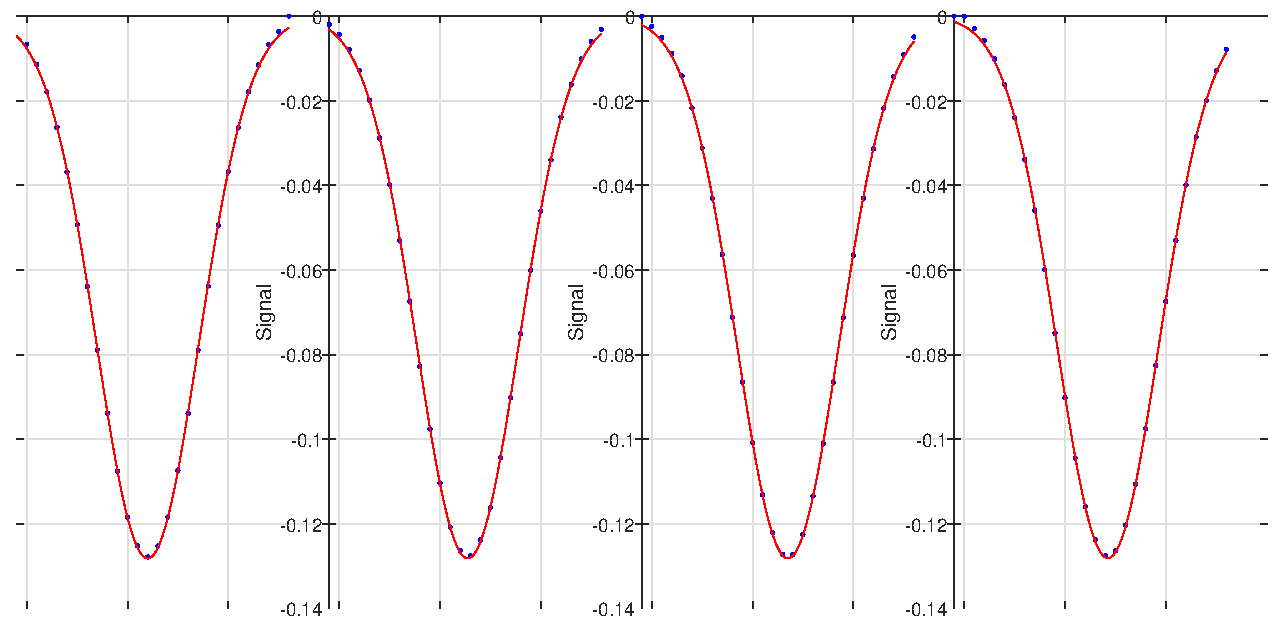
\includegraphics[width = 1\textwidth ]{figures/gaus_sl_4.eps}
    \caption{Gauss Spectral line 4.(absorption) }
    \label{fig:Figure 16}
\end{figure}
\begin{figure}[H]
    \centering
    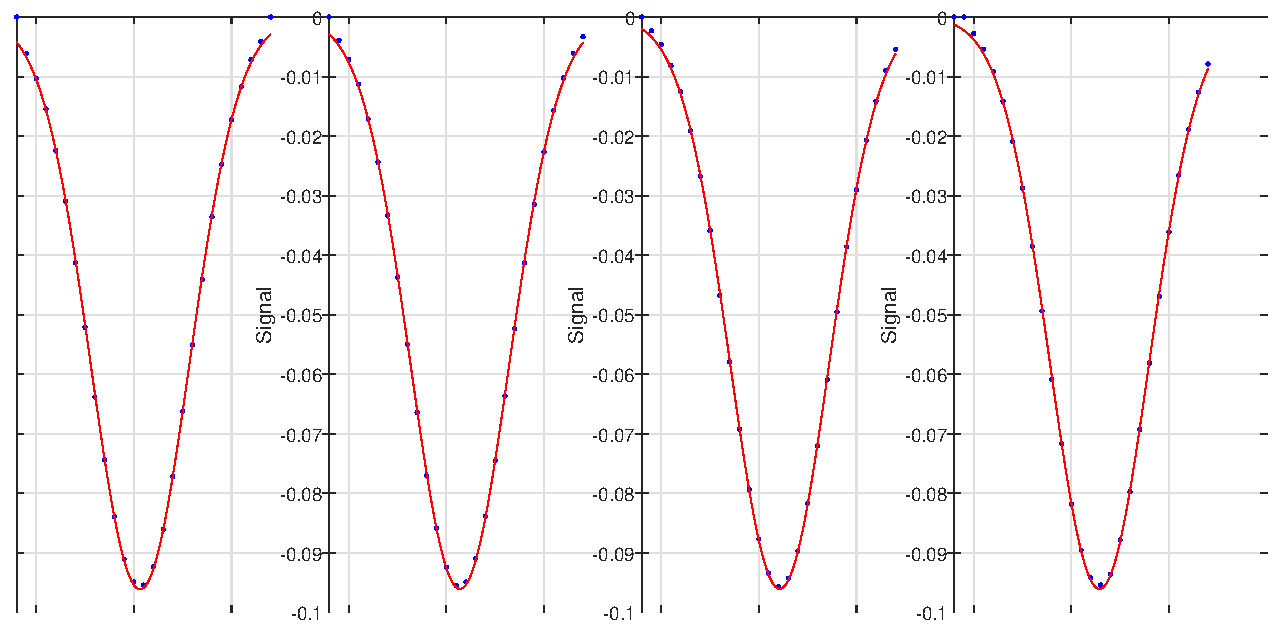
\includegraphics[width = 1\textwidth ]{figures/gaus_sl_5.eps}
    \caption{Gauss Spectral line 5.(absorption) }
    \label{fig:Figure 17}
\end{figure}
\begin{figure}[H]
    \centering
    \includegraphics[width = 1\textwidth ]{figures/gaus_sl_6.eps}
    \caption{Gauss Spectral line 6.(absorption) }
    \label{fig:Figure 18}
\end{figure}
\begin{figure}[H]
    \centering
    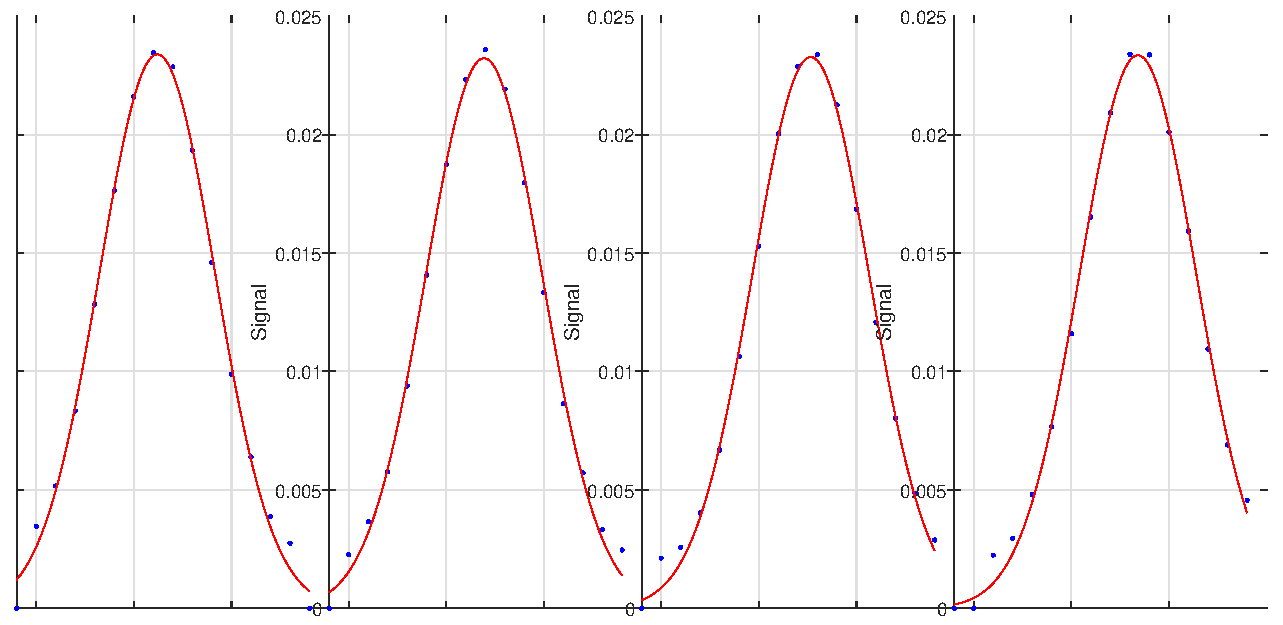
\includegraphics[width = 1\textwidth ]{figures/gaus_sl_7.eps}
    \caption{Gauss Spectral line 7.(emission) }
    \label{fig:Figure 19}
\end{figure}
\begin{figure}[H]
    \centering
    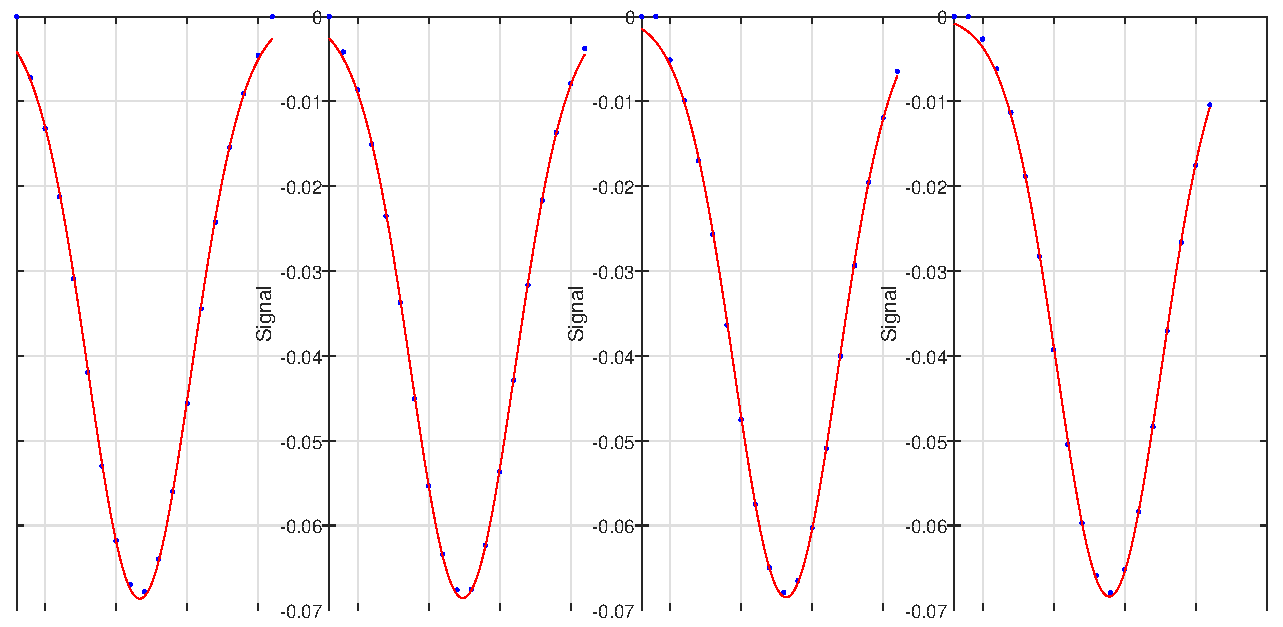
\includegraphics[width = 1\textwidth ]{figures/gaus_sl_8.eps}
    \caption{Gauss Spectral line 8.(absorption) }
    \label{fig:Figure 20}
\end{figure}
\label{endOfDoc}
\end{document}
